\chapter{Descripción del proyecto}
En este capítulo se describe cómo funciona el motor en esencia, es decir, sin entrar en la implementación del mismo. Esta idea general no depende del lenguaje de programación.

Hay un apartado que describe al motor y sus capacidades, y otro apartado que muestra el diseño actual de la aplicación y expone otras ideas que se pueden llevar a cabo.

\section{Qué es Historias del Laberinto (Descripción)}
Historias del Laberinto es una aplicación que funciona como \textbf{intérprete de videojuegos}. Los posibles nombres con los que se identifica al motor en este trabajo son motor, intérprete, aplicación o proyecto.

Esta aplicación permite a un usuario reproducir un videojuego definido en un formato predefinido. Este formato permite abstraer de toda la capa programática a un diseñador.
De momento solo es capaz de reproducir videojuegos, no es capaz de crearlos, aunque en una futura versión probablemente se desarrolle esta opción.

Se ha referido antes al proyecto también como un motor de videojuegos, que se puede definir de esta manera:
\begin{quote}
	\small Un motor de videojuego es un término que hace referencia a una serie de librerías de programación que permiten el diseño, la creación y la representación de un videojuego. \cite{Alberto_Carrasco}
\end{quote}

En el caso de este trabajo, el proyecto no es una serie de librerías sino que es directamente una aplicación. De esta manera, se puede abstraer a un creador del videojuego de la programación directa de un juego.

Otros motores de videojuego que ahora están en el mercado y tienen una funcionalidad similar son Unreal Engine\cite{unrealEngineHomepage} o Unity\cite{unity3dHomepage}. Estos motores permiten crear videojuegos con una capacidad genérica muy potente, pero en muchos casos necesitan que el diseñador tenga conocimientos de diseño 3D, programación y matemáticas. No se ha conseguido llegar al nivel de estos motores, porque supondría un reto muy grande para el ámbito de un trabajo de fin de grado.

\begin{figure}[h]
	\caption{Logo del motor Unreal engine}
	\centering
	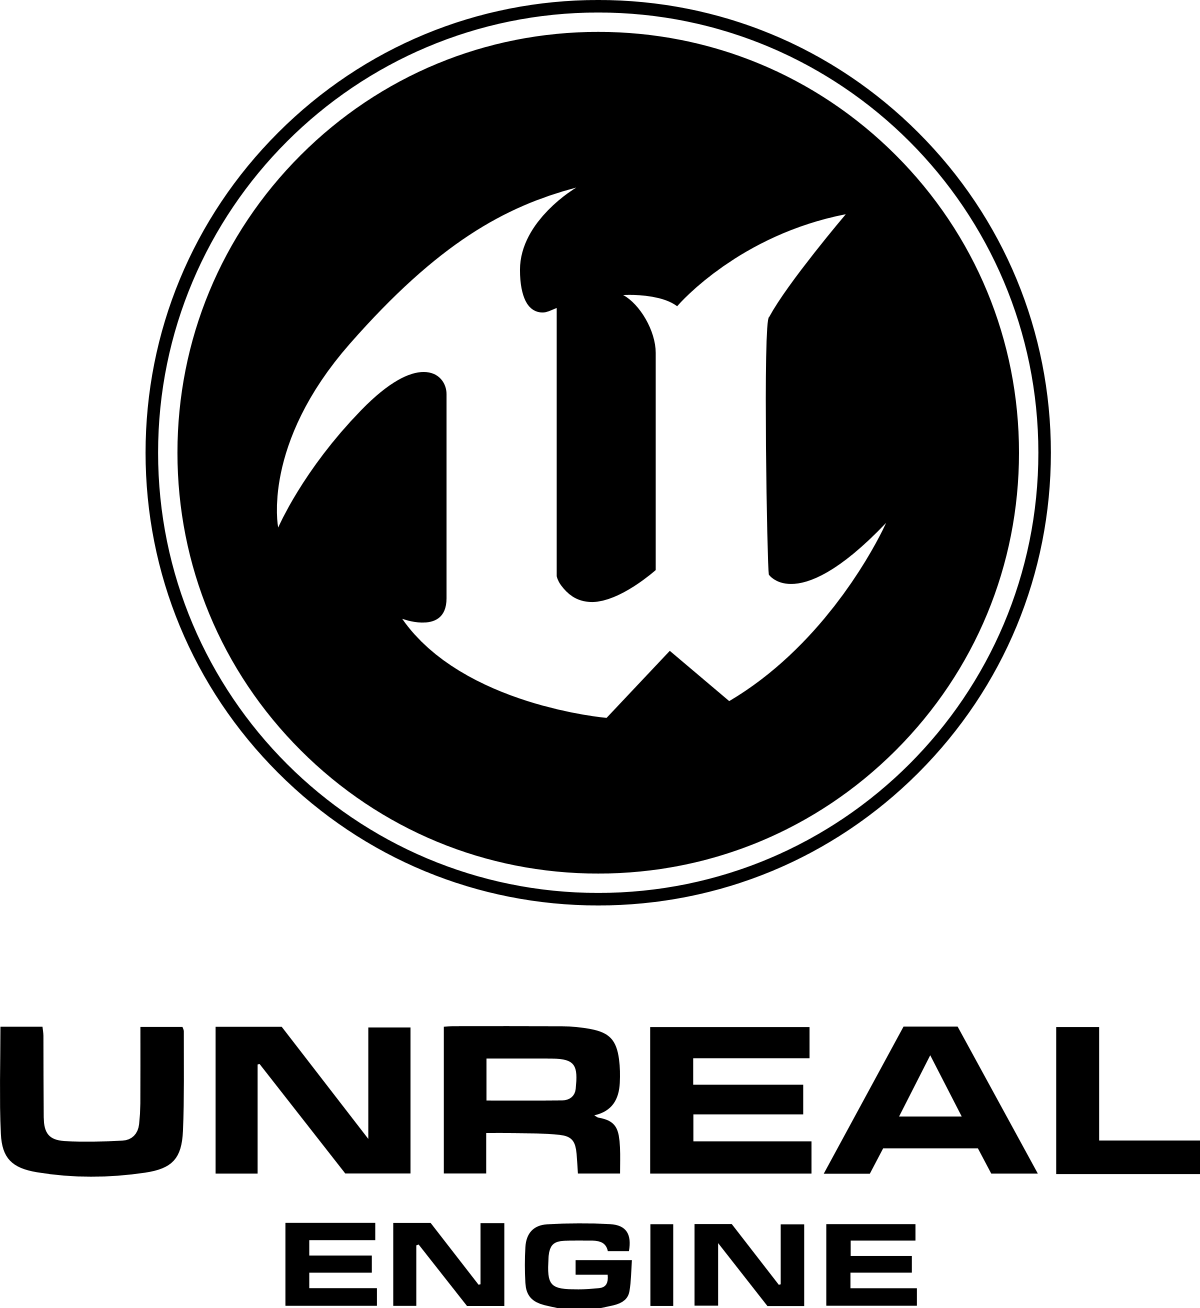
\includegraphics[width=0.3\textwidth]{include/unrealEngineLogo.png}
\end{figure}

\subsection{Qué tipo de videojuegos se pueden crear}
El interprete está orientado a reproducir juegos en los que el jugador tiene que escapar de una mazmorra. Para ello, el jugador debe reunir objetos como llaves para abrir puertas, esquivar trampas, resolver rompecabezas, luchar contra monstruos, usar pociones y llegar a una habitación final.
Algunos ejemplos de juegos parecidos a los que está orientado el motor son ''Dragones y Mazmorras'' o los libros de ''elige tu propia aventura''.

Aunque el motor esté desarrollado con una fuerte influencia por este tipo de juegos, no está limitado a ellos, cualquier creador pueda ir más allá de este concepto o incluso cambiarlo radicalmente usando las herramientas genéricas de las que dispone el motor. El límite lo pone la imaginación del usuario.

\subsection{Dónde se podrá usar el motor}
De momento sólo está disponible para dispositivos que soporten el sistema operativo iOS, es decir, solo para dispositivos portables de Apple, como un iPhone o un iPad.
Tampoco hay planes actuales de mover el motor a otra plataforma, pero es posible implementar el motor en otros sistemas y lenguajes de programación.

Con todas estas dudas resueltas ya solo queda mostrar las funciones de las que dispone el motor.

\subsection{Qué es capaz de hacer el motor}
El proyecto anterior se considera un punto de partida para muchos conceptos que se querían llevar a cabo para el nuevo motor. Por ello, se escogieron ciertas funcionalidades comunes que permitieran representar al videojuego original, separandolas en pequeñas piezas: mostrar un diálogo, iniciar un combate...
De esta manera nacen los \textbf{eventos}.

El juego original también contaba con una serie de jugadores con los que podía interactuar el usuario, salas en las que se desarrollaba la historia, un sistema de movimiento en forma de cuadrícula... Todos estos aspectos se han traducido al motor de manera que sean lo más fieles posibles al juego original.

A continuación, se describen por partes las funcionalidades que tiene el motor. De momento no se entra en las especificaciones propias de la implementación, pero aparecerá el diseño llevado a cabo en la sección \ref{designSection}, y cómo se ha implementado en el capítulo \ref{applicationImplementation}.

\subsection{Eventos}
Un evento representa una acción atómica que puede realizar el motor. Estas acciones se consideran básicas en el ámbito de una aventura, como escoger una opción o mostrar un diálogo; aunque requieran de más trabajo a la hora de programarlas.

Los eventos están pensados para unirse entre ellos, de manera que se puedan mezclar entre sí varias acciones básicas para formar una cadena de eventos. Por ello, cualquiera de ellos son intercambiables, intercalables y no pueden tener dependencias entre sí.
Además, siempre se ejecutan de forma lineal, siguiendo un orden predefinido por el creador del juego.

El centro de toda la potencia del motor reside en los eventos, ya que son un mecanismo genérico y preciso de ejecutar acciones en el juego. El motor está encargado de leer cada uno de estos eventos y ejecutar una acción según el contenido del mismo.
Otra funcionalidad clave del motor es que nunca sabe el estado en el que se encuentra la cadena de eventos, se conforma con guardar el evento que esté ejecutando en el momento, ejecutarlo y pasar al siguiente.

\begin{figure}[h]
	\caption{Cadena de eventos}
	\centering
	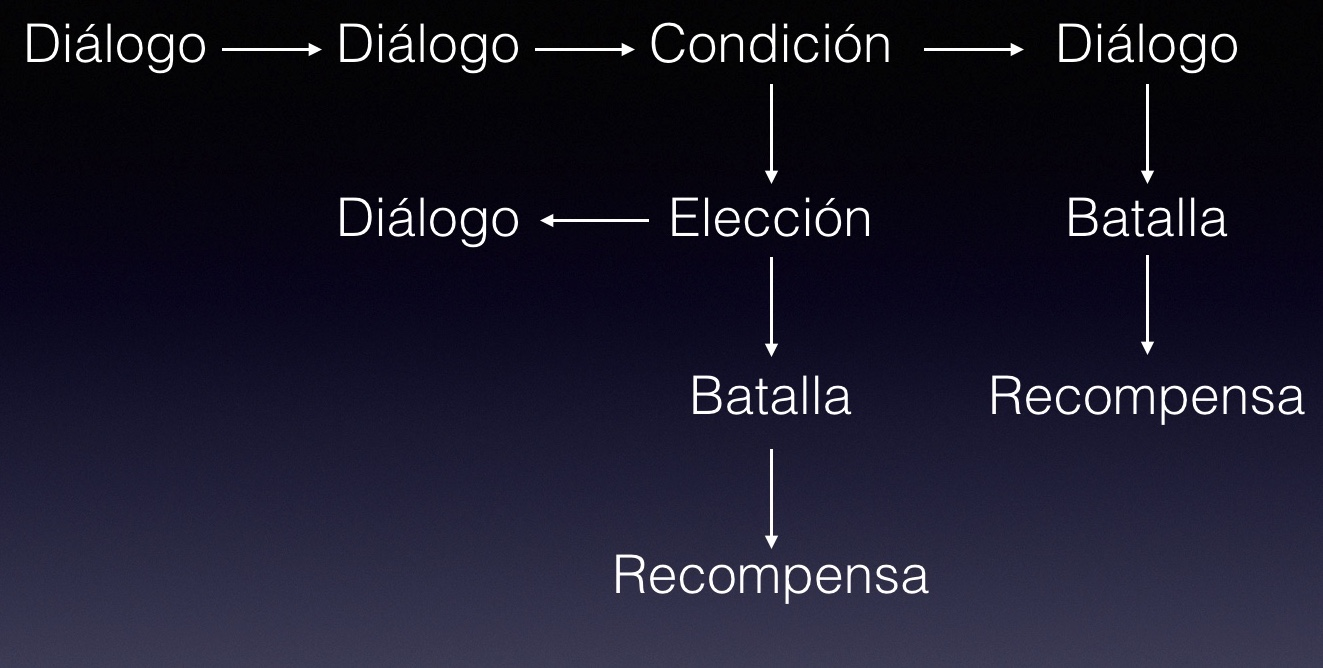
\includegraphics[width=0.75\textwidth]{include/eventsChainExample.jpg}
	
	La idea detrás de los eventos es muy sencilla: al interactuar el usuario con una parte de la aplicación activa una cadena. El evento principal tiene una referencia a otro evento, al que le da paso cuando termina el original. Este encadenamiento sigue hasta que uno de los eventos no tenga ninguna referencia a un evento siguiente, permitiendo que la cadena termine.
\end{figure}

Ahora vamos a definir los tipos de eventos que existen, las acciones que conllevan dentro del motor y sus posibles usos. Respecto a diseño que toman, se describirá más adelante en la sección de diseño \ref{designSection}. 

\subsubsection{Diálogo}
Evento que muestra un mensaje dicho por un personaje en el videojuego. La mayor traba del proyecto original era que los diálogos correspondían con la mayor parte del código fuente, por lo que este evento permite quitar mucha lógica duplicada en el código.

Su uso más frecuente es para mostrar conversaciones entre personajes, aunque también se puede usar para escribir los pensamientos del protagonista, describir una sala o un personaje, plantear un problema...

\subsubsection{Condición}
Evento que verifica una condición sobre el estado actual del juego. Este evento es transparente para el usuario, ya que se ejecutará un evento u otro siguiente dependiendo de si la condición es cierta o no. Las condiciones son las que se describen en la sección \ref{conditionsSubsection}.

Este evento se suele usar cuando se quiere evaluar el estado del juego y tomar acciones en consecuencia. Por ejemplo, diálogos dependientes del compañero, cofres que no se abren si no dispones de una llave...

\subsubsection{Elección}
Evento que permite al jugador escoger entre una serie de opciones. Dependiendo de la opción escogida, se ejecutará un evento u otro. Además, las opciones pueden incluir una condición para que se muestren, como las descritas en la sección \ref{conditionsSubsection}.

Algunos ejemplos en los que aparece este evento son cuando hay que resolver un acertijo y se muestran varias respuestas, o cuando un personaje te ofrece posibles formas de pago para un trueque.

\subsubsection{Batalla}
Evento que inicia una nueva batalla con la información de un enemigo al que enfrentarse.
Hasta que no termine la batalla no se pasará al siguiente evento de la cadena.

Al terminar la batalla se ejecutará un evento según si el jugador ha ganado o ha perdido.

\subsubsection{Recompensa}
Evento que agrega objetos al inventario del jugador.
Se suele usar para recompensar a un jugador por haber ganado una batalla o por haber abierto un cofre.

\subsection{Habitaciones}
La idea original para el desarrollo del juego es un laberinto. Un laberinto se puede representar como una serie de pasillos delgados y oscuros por los que el protagonista debe orientarse, o como una serie de habitaciones interconectadas entre sí.
Esta última opción permite al jugador orientarse por cada partida, obtener mayor detalle sobre los eventos, recordar lugares memorables y ayudar a estructurar el laberinto para el usuario. 

Una habitación es el sitio donde ocurren todos los eventos que se pueden encontrar en el juego. Es en estos lugares donde el jugador va a tener mayor libertad de movimientos porque es el lugar donde se ejecutan cadenas de eventos, puede ir hacia otras habitaciones o donde puede guardar la partida y cambiar ciertos ajustes.

Está representada con una imagen principal que describe a la habitación junto con un título y una descripción, y una serie de acciones que puede realizar el jugador dentro de ella.

\subsection{Personajes}
Durante la aventura el protagonista puede interactuar con múltiples personajes: compañeros, enemigos y NPCs, las siglas de \textit{''non playable character''}. \cite{npcGeekno} Además, el jugador también cuenta como un personaje aparte.

Todos los personajes cuentan con un nombre y una imagen que los representa, y los compañeros y enemigos añaden una serie de características.
Las posibles estadísticas que puede tener un personaje son:

\begin{itemize}
	\item \textbf{Puntos de vida actuales}: representan la vida restante del personaje. Si los puntos de vida actuales del protagonista llegan a 0, entonces el juego termina.
	\item \textbf{Puntos de vida totales}: representan la vida máxima que tiene un personaje.
	\item \textbf{Puntos de ataque}: representan los puntos de vida actuales que puede quitar un personaje con un ataque.
	\item \textbf{Puntos de defensa}: representan los puntos de vida actuales que el personaje elimina de un ataque al recibirlo.
	\item \textbf{Puntos de agilidad}: representan la velocidad de un personaje. En un combate, si un personaje supera por un factor multiplicativo la agilidad del contrario, entonces el personaje puede atacar múltiples veces en un mismo turno. 
	\item \textbf{Estado alterado}: representa un cambio en el estado normal del personaje y pueden reportar beneficios o perjuicios al mismo. Los estados soportados por el motor son veneno, ceguera y parálisis.
	\item \textbf{Arma}: un personaje puede tener un arma consigo para atacar. Estas armas aumentarán el estado base de ataque, añadirán un porcentaje de acierto del ataque y un estado alterado a provocar.
\end{itemize}

Respecto a las tres últimas estadísticas, se explican con más detalle en el apartado de batalla de la sección de diseño \ref{battleDesignSubsection}.

Los personajes por lo tanto son piezas esenciales de la acción durante el juego por distintas razones:

\begin{itemize}
	\item Los diálogos siempre son enunciados por alguien, que debe ser un personaje. Un diálogo no se puede ejecutar si no existe un personaje que lo enuncie.
	\item El protagonista y su compañero tienen una serie de características que son cruciales para la evaluación de condiciones, como los indicadores de habitaciones visitadas.
	\item En una batalla, siempre lucha un personaje enemigo contra el protagonista y sus compañeros.
\end{itemize}

Además, usar personajes permite que los jugadores puedan adentrarse en la aventura con mayor facilidad e incluso identificarse con ellos.

\subsection{Condiciones} \label{conditionsSubsection}
El motor tiene varios puntos donde se necesita ejecutar condiciones para resolver ciertas acciones. Estas condiciones están sujetas a varios factores como las estadísticas del protagonista, valor de las variables internas, etc.

Existen varios tipos de evaluaciones:
\begin{itemize}
	\item Compañero: si el protagonista tiene un compañero que coincide con el nombre definido, entonces la condición se evalúa a verdadera. En otro caso, la condición es falsa.
	\item Objeto: si el protagonista tiene un objeto en su inventario que coincide con el objeto del evento, entonces la condición es cierta. En otro caso, no se cumple la condición. Es importante puntualizar que si la condición es cierta, entonces el objeto del inventario desaparece o se consume.
	\item Estado de habitación: dependiendo si el protagonista ha visitado una habitación específica o no, la condición se evalúa a cierto o falso. Hay una condición que sirve para saber si se ha visitado una habitación y otra para si no la ha visitado.
	\item Relación de variables: si la relación entre dos variables se cumple, entonces la condición es cierta. En otro caso, la condición es falsa. La relación de variables se describe mejor en la sección \ref{variablesSection}.
\end{itemize}

\subsection{Variables personalizadas} \label{variablesSection}
Esta es una nueva funcionalidad del motor que no se encontraba en la original.

Las variables personalizadas es una capacidad del juego que permite almacenar información dinámica de la partida, sin estar limitados por la propia capacidad de evaluar condiciones del motor. Estas permiten a un diseñador de juegos controlar ciertos aspectos internos del desarrollo del juego como puede ser la activación de un evento o de ciertas elecciones.

Estas variables se pueden usar para guardar la información del estado de ejecución de un evento, almacenar la cantidad de tesoros que ha encontrado el jugador durante su partida...

De esta manera, la capacidad de formular condiciones aumenta drásticamente, ya que no dependen de las que puedan estar definidas en el motor. Es más, el diseñador del juego puede emular cualquier condición de las ya definidas si usa las variables correctamente.

Las variables tienen un id que las identifica, el dato que guarda y el tipo de ese dato. Una variable siempre se crea definiendo estos tres campos.
El motor soporta de momento los tipos entero, que representa números enteros; booleano, que representa valores de verdad como verdadero y falso; y cadena de texto, que son un literal de texto.

Debido a que estas variables son dinámicas, el motor permite no solo sustituir el valor o crear nuevas variables, sino que también permite operaciones entre variables u otros datos estáticos.

Las operaciones estarán formadas por dos variables y la operación que realizan entre ellos. El resultado de la operación siempre se guarda en la primera variable con la que se opera. Las operaciones soportadas por el motor dependen del tipo de dato que guarde la variable, y nunca podrán operarse dos variables con distintos tipos de datos.

\begin{itemize}
	\item Las variables \textbf{enteras} soportan las operaciones sustituir, suma, resta, multiplicación, división entera y módulo/resto.
	\item Las variables \textbf{booleanas} soportan las operaciones sustituir, conjunción, disyunción y negación.
	\item Las variables que son \textbf{cadenas de texto} permiten sustituir el texto o concatenarlo.
\end{itemize}

A continuación se describe lo que realiza cada operación:

\begin{itemize}
	\item \textbf{Sustituir}: modifica el valor anterior de la variable con uno nuevo.
	\item \textbf{Disyunción}: ejecuta la operación disyunción booleana sobre la primera y la segunda variable.
	\item \textbf{Conjunción}: ejecuta la operación conjunción booleana sobre la primera y la segunda variable.
	\item \textbf{Negación}: ejecuta la operación negación booleana sobre la segunda variable.
	\item \textbf{Suma}: suma el valor de la primera variable con el de la segunda.
	\item \textbf{Resta}: resta el valor de la primera variable con el de la segunda.
	\item \textbf{Multiplicación}: multiplica el valor de la primera variable por el de la segunda.
	\item \textbf{División entera}: realiza la división entera del valor de la primera variable con el de la segunda.
	\item \textbf{Resto}: halla el resto de la división entera entre el valor de la primera variable y el de la segunda.
	\item \textbf{Sustituir}: concatena el texto de la primera variable con el de la segunda.
\end{itemize}

El uso principal de las variables, cuando ya tienen un valor, es el evaluar su valor comparándolo con otra variable o un dato estático. Para ello, el motor permite realizar operaciones de comparación, y al igual que las operaciones de modificación solo funcionan si los dos tipos de las variables a comparar son iguales. En este caso los operadores son compatibles para todos los tipos de variables, aunque su funcionalidad sea distinta depediendo del tipo.

Los operadores disponibles son igual, distinto, mayor, mayor o igual, menor y menor o igual. A continuación se describe la comparación que se realiza dependiendo del operador.

La condición es cierta:
\begin{itemize}
	\item Operadores enteros:
	\begin{itemize}
		\item \textbf{Igual}: si los dos enteros son iguales.
		\item \textbf{Distinto}: si los dos enteros son distintos.
		\item \textbf{Mayor}: si el primer entero es mayor que el segundo.
		\item \textbf{Mayor o igual}: si el primer entero es mayor que el segundo o si son iguales.
		\item \textbf{Menor}: si el primer entero es menor que el segundo.
		\item \textbf{Menor o igual}: si el primer entero es menor que el segundo o si son iguales.
	\end{itemize}
	\item Operadores booleanos:
	\begin{itemize}
		\item \textbf{Igual}: si los dos valores son iguales.
		\item \textbf{Distinto}: si los dos valores son distintos.
		\item \textbf{Mayor}: si el primer valor es verdadero y el segundo es falso.
		\item \textbf{Mayor o igual}: si el primero es verdadero o si los dos son falsos.
		\item \textbf{Menor}: si el primero es falso y el segundo es verdadero.
		\item \textbf{Menor o igual}: si el primero es falso o si los dos son verdaderos.
	\end{itemize}
	\item Operadores de cadenas de texto:
	\begin{itemize}
		\item \textbf{Igual}: si las dos cadenas son iguales.
		\item \textbf{Distinto}: si las dos cadenas son distintas.
		\item \textbf{Mayor}: si la primera cadena se sitúa posteriormente a la otra según el orden lexicográfico.
		\item \textbf{Mayor o igual}: si la primera cadena se sitúa posteriormente a la otra según el orden lexicográfico o si las cadenas son iguales.
		\item \textbf{Menor}: si la primera cadena se sitúa anteriormente a la otra según el orden lexicográfico.
		\item \textbf{Menor o igual}: si la primera cadena se sitúa anteriormente a la otra según el orden lexicográfico o si las cadenas son iguales.
	\end{itemize}
\end{itemize}

\subsection{Localización}
Supongamos que un diseñador de juegos quiera hacer llegar su juego a la mayor cantidad de gente posible. Aparte de la barrera de los dispositivos que pueden reproducir ese juego, está la barrera del idioma. Aunque ciertos idiomas sean hablados por gran cantidad de gente alrededor del mundo, qué mejor que procurar un juego en el idioma nativo del jugador.

Para ayudar a los diseñadores con este paso, el motor cuenta con soporte para todos los idiomas recogidos en el estándar ISO 639-1 \cite{iso639-1Codes}. Este sistema se ha elegido porque es el estándar que recoge todos los idiomas de forma genérica, sin tener en cuenta diferencias regionales. 

Para ello existen unos ficheros extra donde se pueden definir ciertas claves para ciertos literales de texto que quieren ser traducidos. De esta manera un diseñador puede añadir idiomas extra incluso una vez ya desarrollado el juego. La forma de implementación se describirá en la sección \ref{developmentGuide}.

De ahora en adelante, si se habla de que una funcionalidad es localizable, significa que puede usar una clave que permita traducir el contenido a un idioma.

\newpage
 
\section{Qué esperar del sistema (Diseño)} \label{designSection}
En un mundo en el que todo el mundo puede acceder a miles de aplicaciones a través de un dispositivo portátil que siempre llevan encima y en el que recibir información es lo primordial, es muy importante el diseño que se tiene que llevar a cabo en una aplicación.

Por ello, al desarrollar una aplicación para un teléfono móvil, uno de los factores clave es que sea muy atractiva, bonita y usable.
En esta sección se describirán las elecciones de diseño que se han llevado a cabo para las funcionalidades visuales del motor, dividiéndolas en pantallas visuales. Están adjuntas capturas de la propia aplicación para ayudar a la comprensión de ciertas decisiones.

\subsection{Pantalla de menú principal}
\begin{center}
	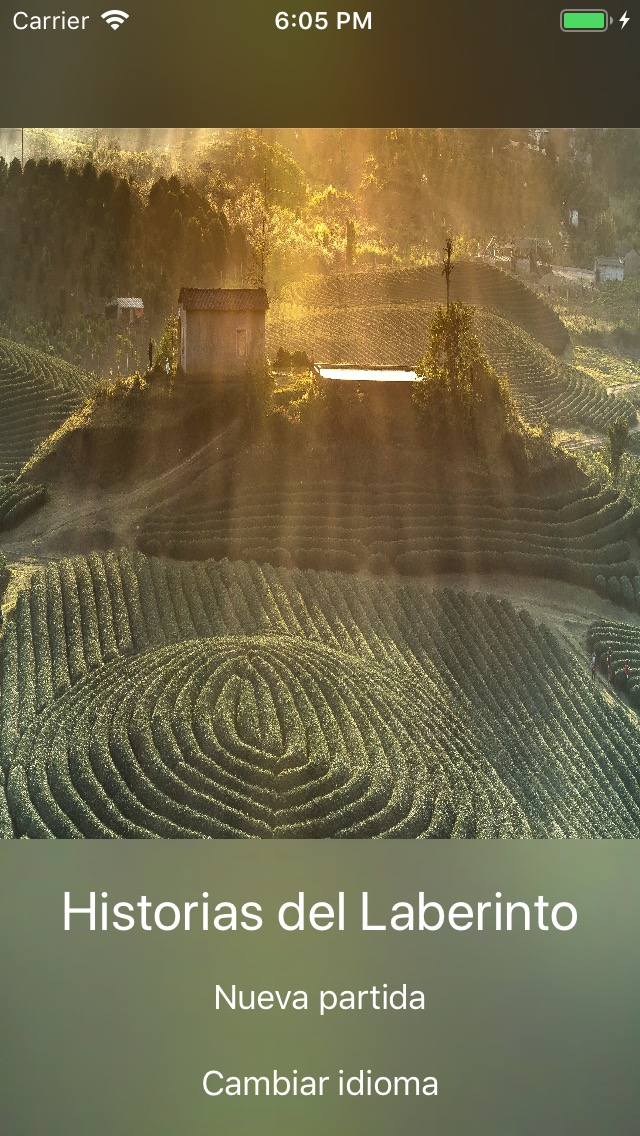
\includegraphics[width=0.3\textwidth]{include/snapshots/mainMenu-es.jpg}
	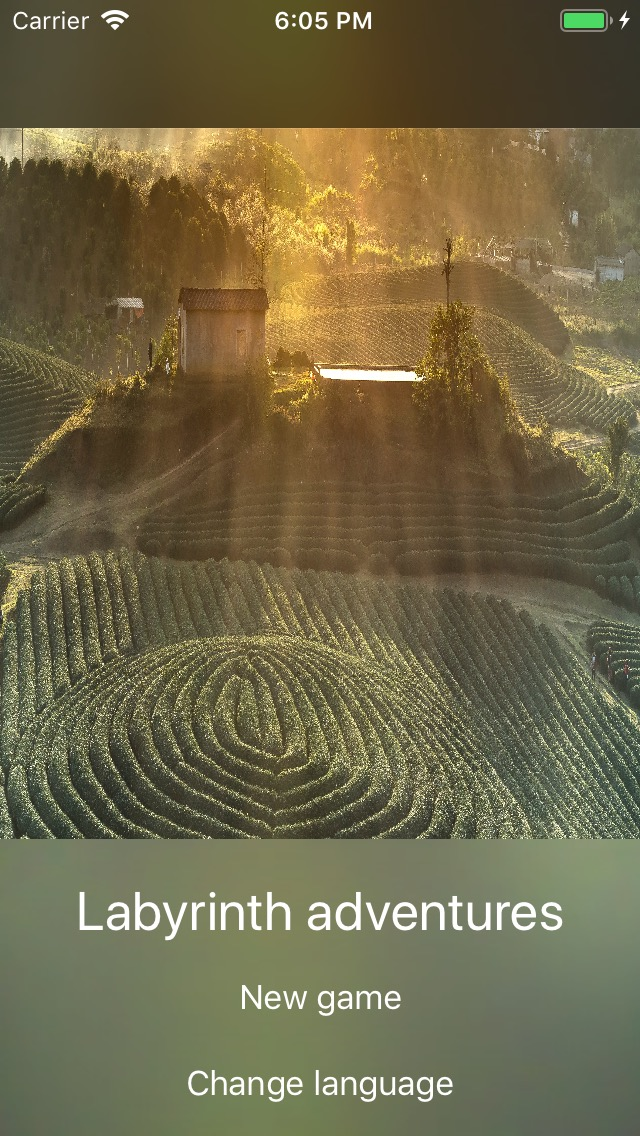
\includegraphics[width=0.3\textwidth]{include/snapshots/mainMenu-en.jpg}
\end{center}
El menú principal es la primera pantalla de la aplicación. Sirve para iniciar la partida cargada, continuar una partida o cambiar el idioma del juego. Debido a que es la primera pantalla del motor, está incluida una imagen con grandes cultivos que asemejan a un laberinto. Esta imagen no se puede cambiar, está fija y no depende del juego cargado.

Nada más cargarse la aplicación, se cargan los ficheros de texto del juego cargado y se escoge un idioma.
El idioma que se elige depende del usuario: si es la primera vez que carga la aplicación, se escogerá uno que corresponda con algún idioma configurado en el dispositivo. En otro caso, usa el lenguaje usado por última vez en la aplicación.

A continuación se describe la acción que debe realizar cada botón:

\begin{itemize}
	\item \textbf{''Nueva partida''}: permite iniciar una nueva partida. Para ello, el motor mostrará una pantalla de carga mientras se encarga de descodificar los ficheros iniciales del juego, guardar la información en la base de datos, inicializar ciertos parámetros y cargar en disco las imágenes que se puedan descargar de Internet.
	\item \textbf{''Cargar partida''}: recupera el estado de una partida guardada anteriormente. Como todos los datos ya están cargados en la base de datos, directamente aparece el lugar en el que estuviera el jugador anteriormente.
	\item \textbf{''Cambiar idioma''}: permite cambiar el idioma de la aplicación. Al pulsar navega directamente a la pantalla de cambio de idioma.
\end{itemize}

\subsection{Pantalla de cambio de idioma}
\begin{center}
	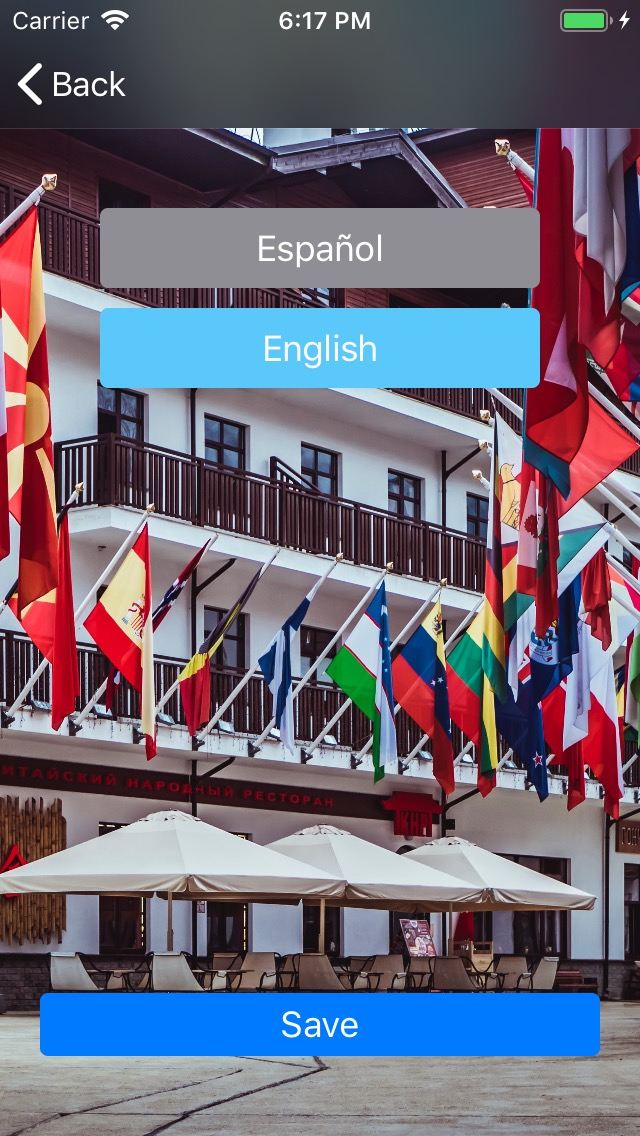
\includegraphics[width=0.3\textwidth]{include/snapshots/languageSettings.jpg}
\end{center}
En esta pantalla se permite al usuario cambiar el idioma entre una lista de idiomas soportados en ese momento por el motor. La aplicación soporta cualquier lenguaje recogido en el estándar ISO 639-1 \cite{iso639-1Codes}.

El fondo no se puede cambiar, aunque muy posiblemente cambie en un futuro muy cercano.
El idioma seleccionado actualmente es el que está marcado en azul. Un jugador puede seleccionar cualquier otro idioma para cambiar la selección, aunque los cambios no se guardan hasta que el usuario pulse el botón de guardado en la parte inferior.
Al pulsar guardar, se recarga la aplicación para que muestre todos los textos en el idioma seleccionado. 

\subsection{Pantalla de habitación}
\begin{center}
	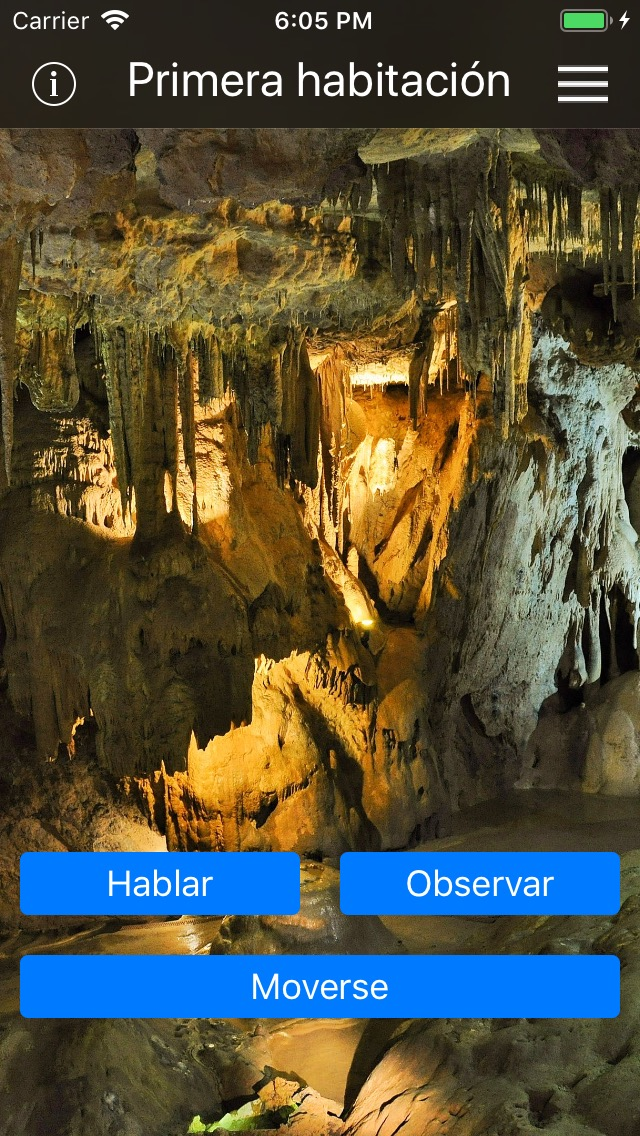
\includegraphics[width=0.3\textwidth]{include/snapshots/roomView.jpg}
	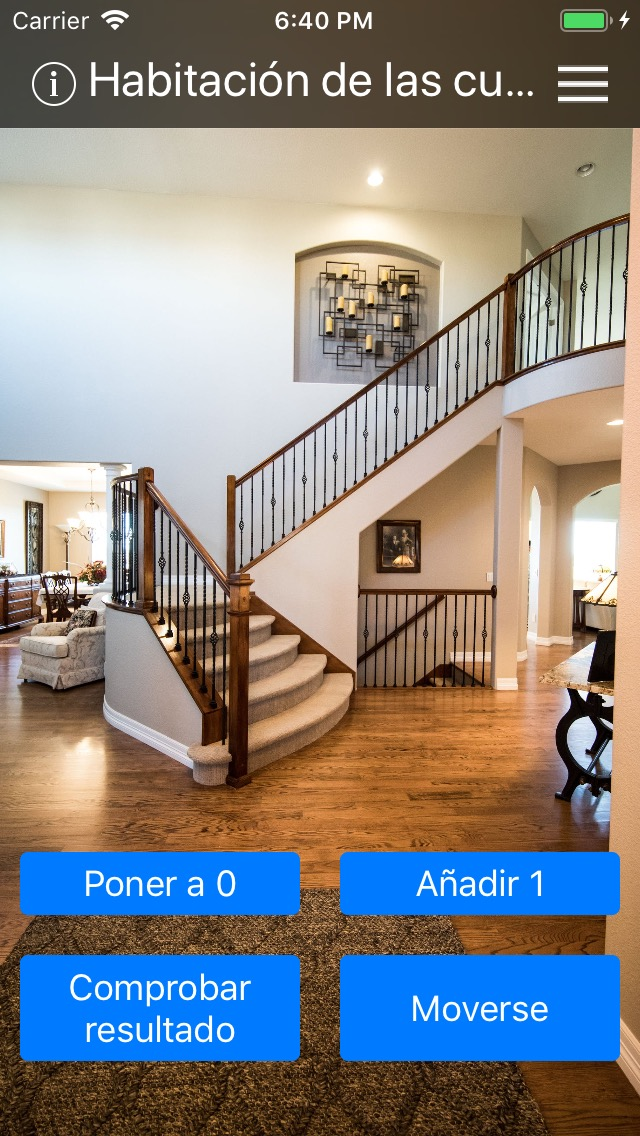
\includegraphics[width=0.3\textwidth]{include/snapshots/secondRoomView.jpg}
\end{center}

La pantalla de habitación es donde se desarrolla la mayor parte de los eventos del juego y es donde el jugador pasará más tiempo en una partida.
Esta pantalla es la encargada de gestionar las acciones principales del jugador: moverse entre otras habitaciones, abrir el menú secundario y ejecutar eventos según una serie de acciones incluidas en la habitación.

La vista cuenta con botones de acción en la parte inferior, un botón de información y un botón de bocadillo. Además el nombre de la misma está escrita en la parte superior, y la imagen de fondo cambia según la habitación en la que se encuentre el usuario.

Esto es lo que ocurre si se pulsan en los distintos botones:
\begin{itemize}
	\item \textbf{Botón de información}: situado en la esquina superior izquierda, el botón de información muestra un diálogo que describe a la habitación en la que se encuentra el jugador.
	\item \textbf{Botón de bocadillo}: situado en la esquina superior derecha, lleva al jugador al menú secundario.
	\item \textbf{Eventos}: las acciones de eventos son los botones azules que siempre están en la parte inferior de la pantalla y representan las acciones que puede realizar el jugador en esa habitación. Al pulsar en uno de ellos, se ejecuta el evento que contenga.
	\item \textbf{''Moverse''}: es el botón azul que está ubicado en la parte inferior de la pantalla como la última acción. Pulsarlo lleva al usuario a la pantalla de movimiento o de cambio de sala.
\end{itemize}

Normalmente una habitación cuenta como máximo con cuatro acciones, incluyendo la de ''Moverse'', aunque soporta muchas acciones, técnicamente infinitas. Cuando aparezcan más de cuatro acciones, entonces la vista de los botones se podrá desplazar para mostrarlos todos.

\subsection{Pantalla de movimiento}
\begin{center}
	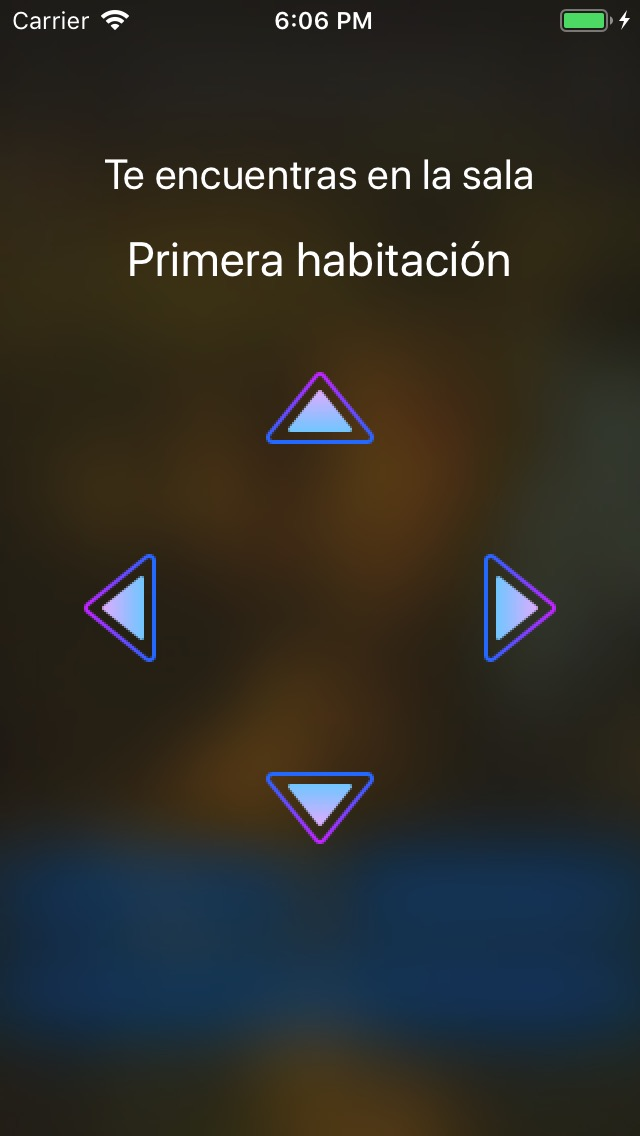
\includegraphics[width=0.3\textwidth]{include/snapshots/movementView.jpg}
	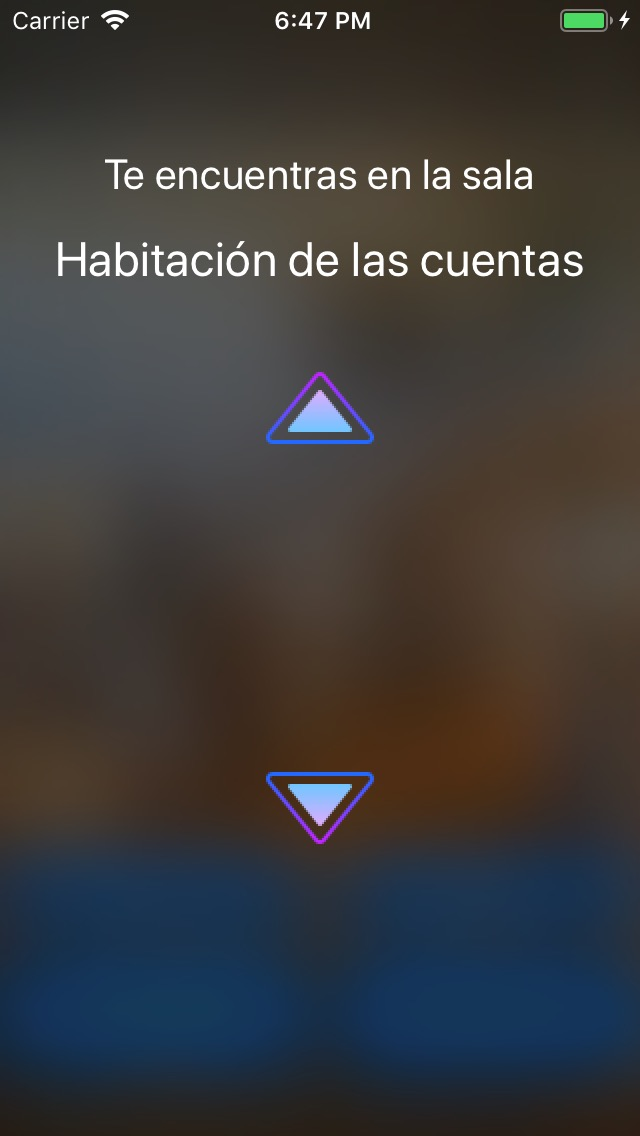
\includegraphics[width=0.3\textwidth]{include/snapshots/movementView_2.jpg}
\end{center}

La pantalla de movimiento permite al jugador cambiar la posición de su personaje y navegar en el laberinto de habitaciones.
Se muestra una pantalla que se superpone a la de la habitación y que contiene el nombre de la habitación en la que se encuentra el usuario y unas flechas que le permiten elegir hacia qué dirección quiere moverse.

Al pulsar en una de las flechas, el jugador se moverá a la habitación que se encuentre en esa dirección, por lo que saldrá de la vista de movimiento y cambiará a la nueva habitación.

El mapa del laberinto es aleatorio, cada vez que el usuario elija una habitación en la que todavía no ha estado presente, el motor recogerá una habitación que no se haya visitado de entre todas las habitaciones configuradas en el juego y fijará su posición, por lo que el jugador podrá volver a visitarla si vuelve al mismo lugar.
Mientras el laberinto tenga varias salas disponibles sin visitar, el movimiento estará disponible en cualquier dirección.
 
En ciertas ocasiones el motor usará una habitación genérica en lugar de las habitaciones configuradas con el propósito de alargar el juego con eventos genéricos determinados por el diseñador. Estas salas normalmente tienen eventos como un cofre con contenido común, un enemigo débil...

Hay que resaltar que en el juego original el jugador cambiaba la dirección a la que miraba cada vez que se movía, simulando un movimiento real de forma más fiel, y para orientarse contaba con una brújula que le permitía saber hacia que punto cardinal estaba mirando.
Sin embargo, en esta aplicación todavía no se ha implementado esta funcionalidad, por lo que no existe este sistema de giro, el jugador siempre estará mirando hacia el mismo sitio.

\subsection{Menú secundario}

\subsection{Inventario}

\subsection{Ejecución de eventos}
La aplicación realiza una acción dependiendo del tipo de evento que se vaya a ejecutar. Algunas de estas acciones muestran una vista que las representa y otras se mantienen invisibles, transparentes para un jugador.

A continuación se describe la acción que realiza cada uno de los eventos, dependiendo del tipo:

\subsubsection{Diálogo}
\begin{center}
	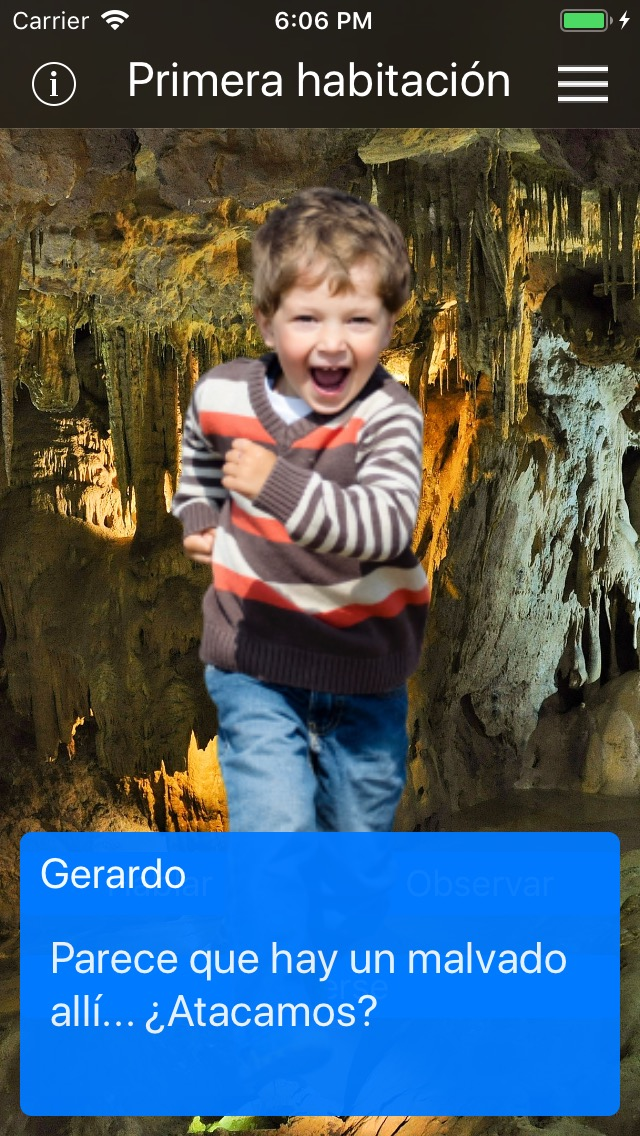
\includegraphics[width=0.3\textwidth]{include/snapshots/dialogue.jpg}
\end{center}
Este evento está encargado de mostrar un mensaje para que el jugador pueda leerlo. Para ello, la aplicación muestra una pantalla por encima de la sala actual, el jugador se mantiene en la misma sala, con ciertas características:

\begin{itemize}
	\item Mensaje: se muestra el mensaje recogido en el evento. Este mensaje es localizable, por lo que se puede traducir a cualquier idioma.
	\item Personaje: se muestra el nombre y la imagen de un personaje, para que el jugador reconozca quién está diciendo el mensaje.
\end{itemize}

Aunque la interfaz de la sala siga viéndose por detrás del diálogo, no se puede interactuar con ella.
Si el usuario pulsa en cualquier sitio de la pantalla, se ejecutará el siguiente evento.

\subsubsection{Condición}
Una condición es un evento transparente para el usuario, no se realizará ningún cambio en la UI. Sin embargo, como realiza operaciones rápidas no bloquea la experiencia de usuario.

\subsubsection{Elección}
\begin{center}
	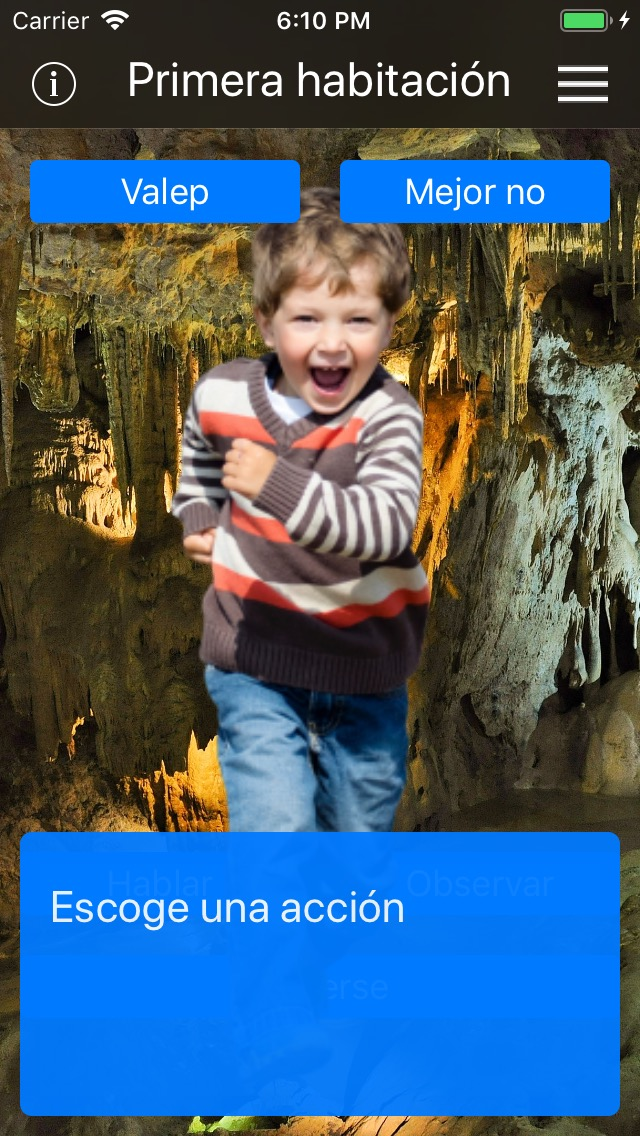
\includegraphics[width=0.3\textwidth]{include/snapshots/chose.jpg}
\end{center}
La elección permite a un usuario recuperar el control de la aplicación y escoger entre una serie de acciones descritas por el evento. Estas opciones aparecen si la condición que tienen anexa se cumple o si no tienen condición.

Muestra un mensaje localizable que insta al jugador a escoger una opción de entre las seleccionadas. Además aparece la imagen del personaje usado en un evento anterior.

El jugador solo puede pulsar en uno de los botones que aparecen con las posibles elecciones. Si el usuario pulsa en cualquier otro sitio, no ocurrirá nada.
Al pulsar en una de estas opciones, se ejecutará el evento que corresponda.

\subsubsection{Batalla} \label{battleDesignSubsection}
\begin{center}
	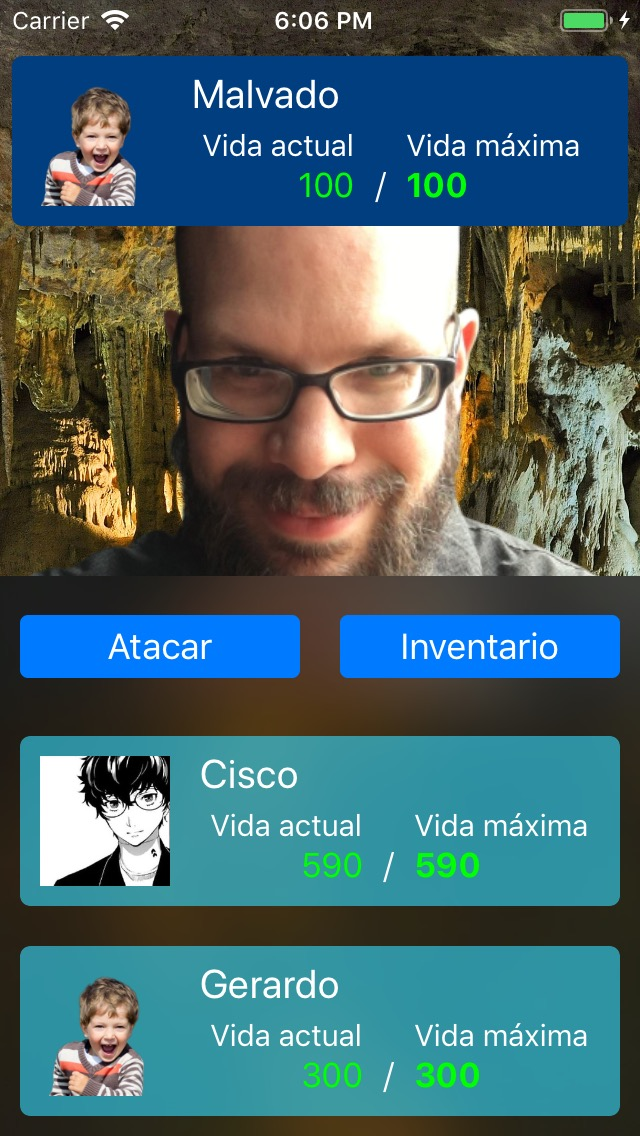
\includegraphics[width=0.3\textwidth]{include/snapshots/battle.jpg}
\end{center}

La batalla es una parte muy importante de la aplicación, ya que es uno de los lugares donde un jugador va a poder salir de la dinámica de explorar la mazmorra y entrar en otra dinámica del juego.
Además, debido a que el planteamiento del combate es muy simple, se necesita que la interfaz sea lo más atractiva posible y que el combate en sí sea suficientemente fluido.

Un combate muestra a dos equipos enfrentados, el equipo del jugador contra el del enemigo. El equipo del jugador tiene que atacar al enemigo y viceversa, reduciendo sus puntos de vida actuales respectivamente. Un luchador se considera derrotado cuando sus puntos de vida actual llegan a 0.

Gana el primer equipo que acabe con el representante del otro equipo, es decir, gana el equipo del enemigo si acaba con el protagonista y gana el equipo del protagonista si acaba con el enemigo principal.

Respecto a la pantalla, debido a que en un combate se representa la lucha entre dos equipos, hay una mitad de pantalla para cada equipo.
En la parte superior se encuentra el bando enemigo. Se muestra una vista de estado con la información del enemigo y una imagen que representa al enemigo principal.
En la parte inferior se encuentra el bando del jugador, mostrando las ventanas con la información de sus luchadores y dos botones que permiten al jugador realizar acciones.

También se puede observar 3 cuadrados de información, dos para el equipo de jugador y uno para el enemigo. En este caso, los dos equipos muestran esencialmente lo mismo. Aquí se describe qué indica cada dato de esta vista:
\begin{itemize}
	\item Nombre y foto del personaje: permite reconocer a cada luchador en la batalla. Cada luchador debería tener su propio nombre y foto para evitar confundir al jugador.
	\item Vida actual: representa la vida actual de la que dispone en el momento el luchador. Esta se reduce si un luchador contrario ataca al luchador, por lo tanto el número varía.
	Además, los puntos de vida siguen un código de colores para ayudar al jugador a darse cuenta del estado en el que se encuentra ese luchador: si el color es \textcolor{green}{verde} significa que los puntos de vida actuales están al máximo, si el color es \textcolor{yellow}{amarillo} significa que los puntos están por debajo de un cuarto del máximo, si el color es  \textcolor{red}{rojo} significa que tiene 0 puntos, y en otro caso el color será blanco.
	\item Vida máxima: representa el tope de vida que tiene un luchador.
	\item Estado alterado: situado en la esquina superior derecha, representa el estado alterado que puede sufrir uno de los personajes. Si el personaje no tiene ningún estado alterado, entonces no aparece información al respecto.
\end{itemize}

Durante una batalla, el jugador solamente podrá controlar a su personaje, al protagonista. El resto de acciones, las realizadas por el resto del equipo del jugador y el equipo del enemigo, son calculadas automáticamente por la aplicación. 

Respecto a las dos botones, representan las dos acciones que puede realizar un usuario.
\begin{itemize}
	\item Atacar: realiza la acción de atacar sobre el enemigo.
	\item Inventario: lleva al usuario a la vista de inventario, para permitirle usar objetos de la misma manera que desde el menú secundario.
\end{itemize}

La batalla está diseñada prácticamente igual a la que se encontraba en el juego original. Aunque esta vez la aplicación cuente con una interfaz que representa mejor una pelea, el núcleo lógico de toda la pantalla es muy parecido al anterior. De todas maneras, a continuación se describe cómo está diseñada la vista, funcionalmente hablando. 

El combate sigue siendo por turnos, siguiendo el orden original: primero actúa el protagonista, después el enemigo y por último el resto del equipo del jugador. Cada turno cuenta con una serie de fases que le permite al jugador darse cuenta de lo que está ocurriendo. En esta descripción, siempre se hablará del personaje que actúa en el turno como luchador y contrario como el personaje al que ataca el responsable del turno.

\begin{enumerate}
	\item Fase de continuidad de estado alterado: el motor analiza el estado del luchador, y si tiene un estado alterado evalúa que el luchador pueda perder ese estado alterado.
	\item Fase de evaluación de daño de estado alterado: el motor analiza el estado del luchador y realiza ciertas acciones si tiene un estado alterado específico. Si el luchador está envenenado, entonces le hace una cantidad de daño al luchador; y si está paralizado hay una probabilidad de que pierda su turno.
	\item Fase de introducción de acción: el motor pregunta al luchador qué acción quiere realizar. Si el luchador es el protagonista, el jugador podrá elegir una de las acciones descritas anteriormente en los botones. En otro caso, el luchador siempre decidirá atacar al contrario.
	\item Fase de ataque: el motor comienza el cálculo del ataque. Si no se dispone de objetivo, el motor elige uno aleatoriamente del equipo contrario de entre los que están vivos, es decir, tienen más de 0 puntos de vida actuales. Tras ello, el motor calcula el daño que recibe el objetivo a partir de las estadísticas del luchador y el contrario.
	Además, si el luchador cuenta con el estado alterado ceguera, entonces es posible que falle el ataque.
	\item Fase de evaluación de daño contrario: el motor analiza el estado del contrario y evalúa si está derrotado.
\end{enumerate}

Esta cadena de turnos se repite hasta que se da el caso de que uno de los representantes de los equipos sea derrotado. Si el representante del equipo enemigo ha sido derrotado, entonces se activa el evento de victoria. Si el protagonista es el derrotado, entonces se activa el evento de derrota.

\subsubsection{Recompensa}
\begin{center}
	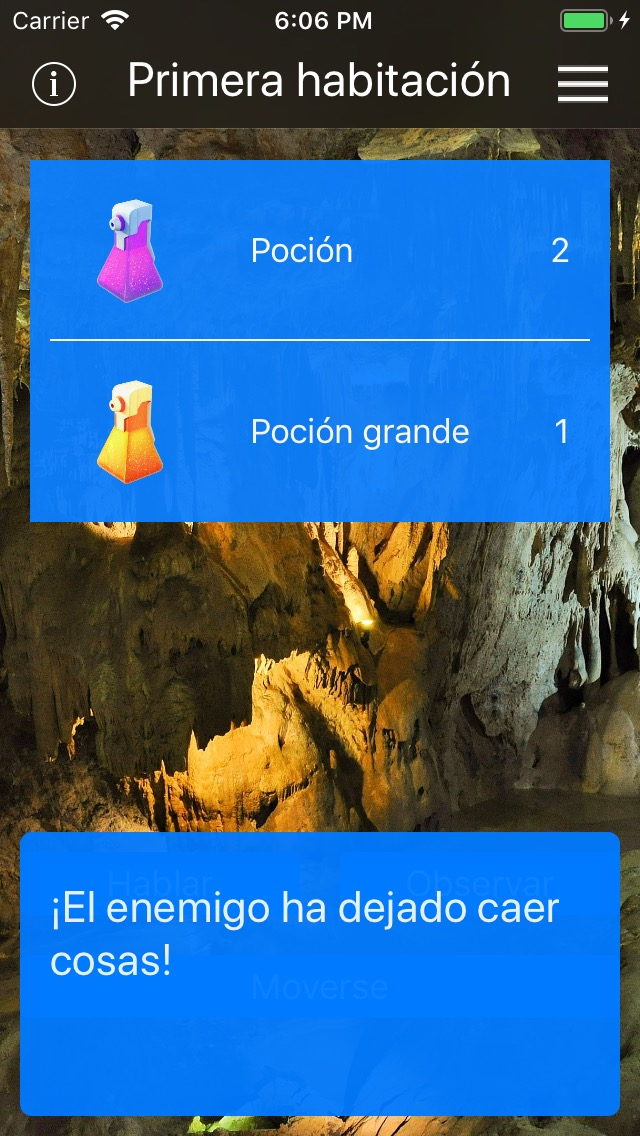
\includegraphics[width=0.3\textwidth]{include/snapshots/reward.jpg}
\end{center}
La recompensa muestra al usuario una serie de objetos que consigue, especificados en el evento.
En la parte inferior se muestra un mensaje localizable del evento. En la parte superior se muestra una lista de objetos obtenidos por el jugador. Teóricamente un jugador puede recibir tantos objetos como se especifique en el evento.
Cada objeto está representado con su nombre localizable, una cantidad que se recibe y una foto indicando qué objetos se reciben.

\section{Cómo crear un videojuego} \label{developmentGuide}
En esta sección se define cómo crear un juego que sea compatible con el motor. Para ello, se dispone de una serie de ficheros que permiten a la aplicación cargar la información básica y empezar el juego. En esta sección se explicará para qué sirve cada fichero y cómo se deben rellenar.

Estos ficheros tienen formato YAML \cite{yamlDocumentation}. Este formato permite la manipulación de datos serializables de forma sencilla tanto por el programador como por un usuario, es decir, son ficheros fáciles de transformar a código y son fáciles de interpretar y diseñar por una persona.

Todas las claves están definidas en inglés, para permitir que los diseñadores puedan tener un lenguaje común para crear juegos.

\subsection{Imágenes}
Un diseñador puede crear o descargar sus propias imágenes para usarlas en el juego. Para ello existe una carpeta llamada ''images'', donde se deben guardar las imágenes necesarias.
En todo caso, si el diseñador prefiere generar un juego de manera que sus elementos no pesen demasiado, el motor también soporta la descarga de imágenes por Internet, siempre teniendo en cuenta que sólo puede descargar imágenes de URLs con soporte SSL a través del protocolo HTTPS, es decir, que comiencen por ''https''.
El motor acepta archivos con tipos comunes, como JPEG o PNG. No se asegura la compatibilidad con otros tipos de ficheros.

Para representar una imagen hay que especificar el origen de la imagen y el lugar donde se encuentra el recurso. El origen puede ser tanto local como remoto. Si el origen es local, el diseñador debe especificar el nombre del fichero al que quiere acceder. Si el origen es remoto, el diseñador debe especificar la URL que contiene la imagen. 

\begin{lstlisting}[style=Python]
# -*- coding: utf-8 -*-

\end{lstlisting}


\subsection{Literales localizables}
\subsection{Personajes}
\subsection{Protagonista}
\subsection{Objetos}
\subsection{Variables}
\subsection{Habitaciones}
\subsection{Eventos}

Antes de comenzar, todos los eventos tienen una serie de características comunes entre ellos:

\begin{itemize}
	\item Identificador: todos los eventos cuentan con un id, y este debe ser único. No se asegura que dos eventos con identificadores idénticos funcionen a la vez.
	\item Siguiente paso: indica el identificador del próximo evento a ejecutarse...
	akbhdfdkjalskshbebbjdkjbajbkRELLENAR
\end{itemize}

Para crear un videojuego disponemos de x archivos.
Describir cada uno y explicar en qué se traduce en el juego



\chapter{Desarrollo de la aplicación} \label{applicationImplementation}

\section{Una manera de llevarlo a cabo (Arquitectura)}

\section{Desarrollando en dispositivos móviles (Implementación)}

De la forma en la que están desarrollados los eventos en este momento, permite a los desarrolladores de este motor crear nuevos tipos de eventos, sin perjuicio de ninguna implementación de los anteriores.